\documentclass[11pt]{report}
\usepackage{titlesec}
\titleformat{\chapter}
  {\normalfont\LARGE\bfseries}{\thechapter}{1em}{}
\titlespacing*{\chapter}{0pt}{3.5ex plus 1ex minus .2ex}{2.3ex plus .2ex}

\usepackage[margin=1.2in]{geometry}
\usepackage[toc,page]{appendix}
\usepackage{graphicx}
\usepackage{lipsum}
\usepackage{caption}
\usepackage[utf8]{inputenc}
\usepackage[italian]{babel}
\usepackage{verbatim}
\usepackage{colorprofiles}
\usepackage{listings}   %<- per inserire il codice
\usepackage{float}
\usepackage{subcaption}
\usepackage{amsmath}
\usepackage{amsfonts}
\usepackage{listings}
\usepackage{xcolor}

%%%%%%%%%%%%%%%%%%%%%%%%%%%%%%%%%%%%%%%%%%%%%%%%%%%%%%%%%%%%%%%%%%%%
\definecolor{custom_green}{rgb}{0,0.6,0}
\definecolor{codegray}{rgb}{0.5,0.5,0.5}
\definecolor{codepurple}{rgb}{0.58,0,0.82}
\definecolor{backcolour}{rgb}{0.95,0.95,0.92}
\definecolor{custom_blue}{rgb}{  0.05, 0.05, 0.97}
\definecolor{custom_brown}{rgb}{ 0.69, 0.38, 0.10}
\definecolor{custom_purple}{rgb}{0.58, 0.00, 0.82}
\definecolor{custom_orange}{rgb}{0.94, 0.59, 0.09}

\lstdefinestyle{MATLABstyle}{   
    commentstyle=\color{custom_green},
    keywordstyle=\color{magenta},
    numberstyle=\tiny\color{codegray},
    stringstyle=\color{codepurple},
    basicstyle=\ttfamily\footnotesize,
    breakatwhitespace=false,         
    breaklines=true,                 
    captionpos=b,                    
    keepspaces=true,                 
    numbers=left,                    
    numbersep=5pt,                  
    showspaces=false,                
    showstringspaces=false,
    showtabs=false,                  
    tabsize=2
}
\lstdefinelanguage{Cpp}{
      language=C++,
      backgroundcolor=\color{white},  
      basicstyle=\footnotesize \ttfamily \color{black} \bfseries,   
      breakatwhitespace=false,       
      breaklines=true,               
      captionpos=b,                   
      commentstyle=\color{custom_green},   
      deletekeywords={...},          
      escapeinside={\%*}{*)},
      keywordstyle=\color{custom_purple},
      identifierstyle=\color{blue},
      stringstyle=\color{blue},      
      numbers=left,                 
      numbersep=5pt,                  
      numberstyle=\tiny\color{black}, 
      rulecolor=\color{black},        
      showspaces=false,               
      showstringspaces=false,        
      showtabs=false,                
      stepnumber=1,                   
      tabsize=5,                     
      title=\lstname,                 
    }

\lstdefinelanguage{Python}{
    keywords={from, import, def, return, as, in, len, if, elif, else, for, while},
    breakatwhitespace=false,       
    breaklines=true,   
    morecomment=[l]{\#},
    morestring=[b]",
    commentstyle=\color{red},
    keywordstyle=\color{custom_purple},
    numberstyle=\tiny\color{black},
    stringstyle=\color{custom_green},
    basicstyle=\ttfamily\footnotesize,
    captionpos=b,
    showstringspaces=false,        
    showtabs=false,                
    numbers=left,                 
    numbersep=5pt,                  
    numberstyle=\tiny\color{black}, 
    rulecolor=\color{black},                      
    tabsize=5,                     
    title=\lstname,    
}

\lstdefinelanguage{MATLABc}{
    language=MATLAB,
    backgroundcolor=\color{white},  
    basicstyle=\footnotesize \ttfamily \color{black} \bfseries,   
    breakatwhitespace=false,       
    breaklines=true,               
    captionpos=b,
    morestring=[b]",
    commentstyle=\color{custom_green},   
    keywordstyle=\color{custom_blue},
    morekeywords={clearvars},
    deletekeywords={fprintf},
    identifierstyle=\color{black},
    stringstyle=\color{custom_purple},      
    numbers=left,                 
    numbersep=5pt,                  
    numberstyle=\tiny\color{black}, 
    rulecolor=\color{black},        
    showspaces=false,               
    showstringspaces=false,        
    showtabs=false,                
    stepnumber=1,                   
    tabsize=5,                     
    title=\lstname,                 
}
%%%%%%%%%%%%%%%%%%%%%%%%%%%%%%%%%%%%%%%%%%%%%%%%%%%%%%%%%%%%%%%%%%%%




\begin{document}
\captionsetup[figure]{margin=1.5cm,font=small,labelfont={bf},name={Figure},labelsep=colon,textfont={it}}
\captionsetup[table]{margin=1.5cm,font=small,labelfont={bf},name={Table},labelsep=colon,textfont={it}}


\begin{titlepage}
\begin{center}
\LARGE {\scshape{Università Politecnica delle Marche}}\\[0.5cm]
\LARGE {\scshape{Ingegneria Informatica e dell'Automazione}}\\[0.7cm]
\linespread{1}
\huge {\bfseries Titolo significativo }\\[1cm]
\linespread{1}

\includegraphics[width=5cm]{images/logoUnivpm.jpg}\\[0.5cm]
\linespread{1.2}
\Large Corso di\\
\Large {\scshape{Laboratorio di Automazione}} \\[0.3cm]
\Large {Anno accademico 2023-2024 \\[0.8cm]}
{\Large Studenti:}
\hfill {\Large Professore:}\\
{\Large Nome Cognome}
\hfill
{\Large Andrea Bonci}\\
\raggedright{\Large Nome Cognome\\}
\raggedleft{\Large Dottorando:\\
\Large Nome Cognome\\[1cm]}
\centering{

\includegraphics[width=2cm]{images/dii_new.png}\\[0.3cm]
\large Dipartimento di Ingegneria dell'Informazione\\[0.3cm]
}
\end{center}
\end{titlepage}

\pagenumbering{arabic}
\tableofcontents
\addcontentsline{toc}{chapter}{Introduzione}
\newpage

\pagestyle{plain}

\section*{Introduzione}
Spiegazione dettagliata del task assegnato al gruppo (cosa avete fatto e su quale sistema).\\
Se per lo svolgimento del task è stato necessario interagire con altri gruppi che hanno lavorato sullo stesso sistema presentare anche brevemente i task svolti dagli altri gruppi e spiegare la loro interconnessione.
Se si è invece optato per far confluire il lavoro di più gruppi in un'unica relazione, va spiegato qual era il task iniziale dei singoli gruppi e poi come è avvenuta l'integrazione. \\
In sintesi, l'introduzione deve permettere al lettore di capire subito su cosa avete lavorato.
Al termine dell'introduzione inserite anche una breve descrizione per capitoli del contenuto della restante parte della relazione (es Nel Capitolo \ref{Hardware} viene descritto...). \\
\newline
Nel seguito la struttura in capitoli di massima per ogni relazione, da adattare qualora necessario. \\
\textcolor{red}{NOTA: La relazione va pensata e scritta nell'ottica di dare a chi verrà dopo di voi un documento utile per capire a che punto è arrivata l'attività svolta dal vostro gruppo e per metterli in condizione di portare avanti il vostro lavoro. Di conseguenza dovete essere chiari e diretti, riportando solo le informazioni necessarie e evidenziando in modo critico cosa effettivamente funziona correttamente e cosa va migliorato}

\newpage
\chapter{Sistema}
\textcolor{red}{NOTA valido per ogni capitolo: }inserire all'inizio di ogni capitolo una brevissima descrizione del contenuto del capitolo stesso.\\
\newline
\textcolor{red}{NOTA:} capitolo opzionale.
Solo se necessario per comprendere quanto svolto, inserite un capitolo dedicato al sistema su cui avete lavorato (es drone quadrirotore, ballbot ..) dove descrivete ad esempio come è fatto il sistema, come si modella matematicamente e come si può controllare. Nel capitolo inserite solo le informazioni che avete effettivamente utilizzato per svolgere il task assegnatovi (\textcolor{red}{evitate il copia e incolla dalle vecchie relazioni}). Mettete la fonte da cui avete preso le informazioni (es vecchia relazione \cite{Relazione1}).
\section{Modello matematico}
\section{Controllo}

\newpage
\chapter{Hardware}
\label{Hardware}
Inserire sempre un capitolo "Hardware" dove si descrivono tutti i componenti hardware utilizzati (schede, sensori, attuatori..). Dedicare un paragrafo ad ogni componente. Per ogni componente riportare le seguenti informazioni: modello specifico, riferimento bibliografico con link ad un sito web con la documentazione del componente (es \cite{DCdriver}), immagine, pinout, solo le informazioni rilevanti per lo svolgimento del task.
\section{Componente1}
\section{Componente2}
\section{Schema dei collegamenti}
Inserire uno schema dei collegamenti analogo a quello in Figura \ref{fig:schema}. Si suggerisce per lo scopo di usare il software "draw.io". Nello schema riportare tutti i collegamenti tra i componenti, specificando quale pin di un componente1 si collega con quale pin di un componente2 (per la maggior parte dei collegamenti dovete cioè avere una linea con 2 label). \\
Inserire anche una descrizione testuale dello schema.

\begin{figure}[H]
\centering
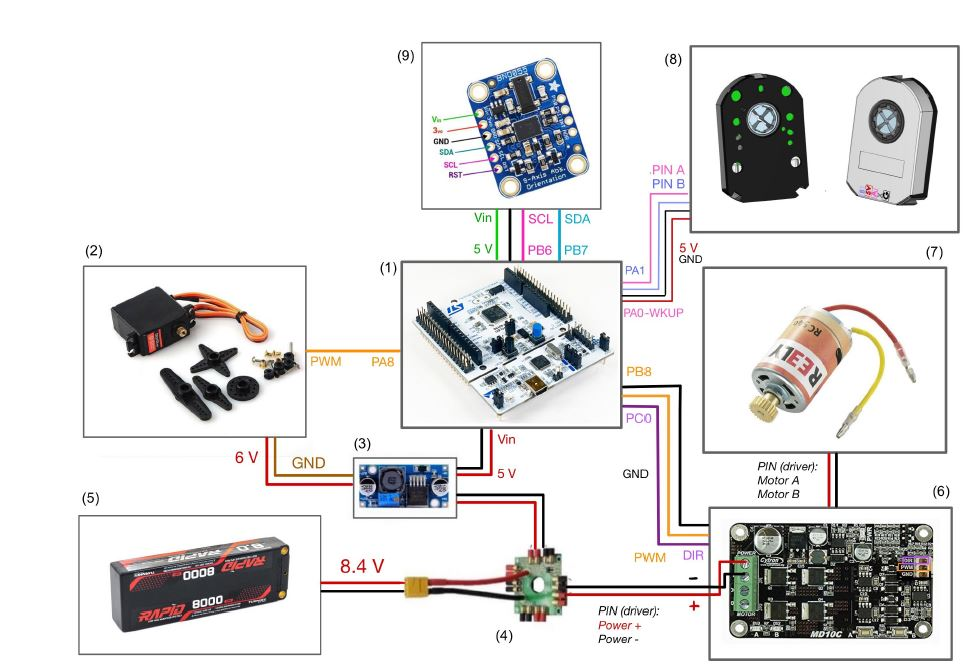
\includegraphics[width=0.8\textwidth,keepaspectratio]{figures/Schema.JPG}
\caption{Schema dei collegamenti}
\label{fig:schema}
\end{figure}


\chapter{Software}
Nell'introduzione al capitolo specificate anche la versione dell'STM32CubeIDE e dell'STM32CubeMX che avete usato (se avete cambiato versione nel corso del progetto mettete l'ultima, quella su cui è sviluppato il codice che consegnate).

\section{Diagramma di flusso}
Inserire un diagramma di flusso analogo a quello in Figura \ref{fig:diagramma} che spiega il funzionamento generale del codice sviluppato. Inserire anche una descrizione testuale del funzionamento.

\begin{figure}[H]
\centering
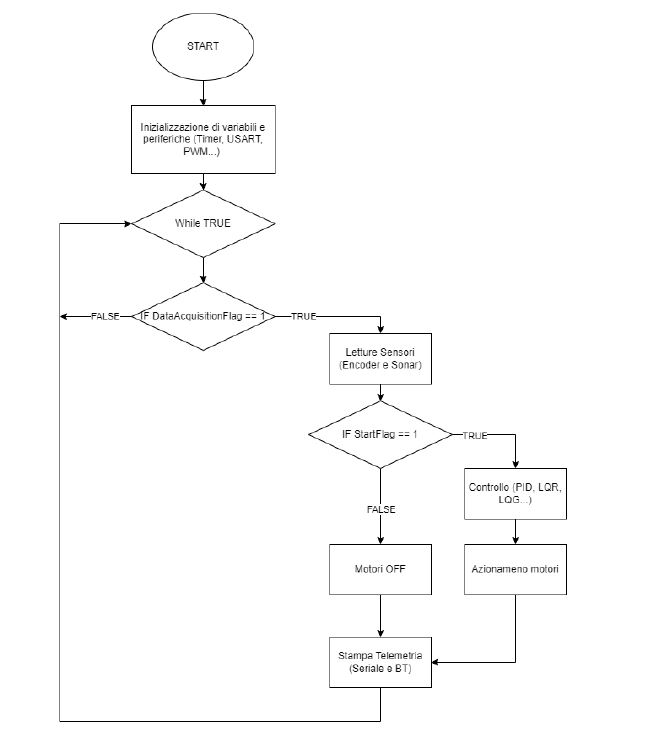
\includegraphics[width=0.8\textwidth,keepaspectratio]{figures/diagramma.JPG}
\caption{Diagramma di flusso del codice sviluppato}
\label{fig:diagramma}
\end{figure}

\section{Gestione singoli componenti}
Dedicare un pagagrafo ad ogni componente in cui viene spiegato il codice che lo gestisce. Inserite prima una descrizione generale di come si gestisce un componente di quel tipo (aiutandovi con schemi o altro). Poi le configurazioni che sono state fatte sul .ioc per poterlo utilizzare (quale periferiche sono state abilitate, come sono state configurate.. mettete degli screen del .ioc). Infine inserite e spiegate le parti di codice che lo gestiscono.\\
\newline
\textcolor{red}{NOTA per il codice}: per rendere il codice modulare e riutilizzabile è buona prassi non caricare troppo il main ma creare una libreria per ogni componente. Quindi il componente1 avrà un header file "componente1.h" e un source file "componente1.c", nel source file sono implementate le funzioni che gestiscono il componente, nell'header file ci sono i prototipi di tali funzioni in modo che esse possano essere usate nel main includendolo.\\
\newline
\textcolor{red}{NOTA per il codice}: non inserire mai nel codice dei parametri numerici senza contesto ma renderli delle costanti definite (usando la direttiva \%define). Se sono delle costanti relative ad uno specifico componente vanno inserite nel relativo header file.\\
\newline
\textcolor{red}{NOTA per il codice}: per inserire il codice, anziché utilizzare screenshot utilizzate i seguenti comandi.\\
Per codice scritto in latex (con linguaggio Python):
\begin{lstlisting}[language=Python, caption="Codice in Python"]
import numpy as np
    
def incmatrix(genl1,genl2):
    m = len(genl1) # The length of the first array
    n = len(genl2) # The length of the second array
    sum = 0
    
    # Compute 
    for i in range(0,n):
        for j in range(0, m):
            sum += genl1[n]*genl2[m]

    # Print
    print("The sum is %2d" %(sum))   
    
    return M
\end{lstlisting}
Per codice richiamato da file (con linguaggio C):

\lstinputlisting[language=Cpp, firstline=4, lastline=8, caption="Codice in C"]{codefiles/example_code.cpp}

Funziona anche per codice MATLAB:
\begin{lstlisting}[language=MATLABc, caption="Codice in MATLAB"]
%% PREPARE WORKSPACE
close all
clearvars
clc

%% OPERATIONS
sayhello;

%% FUNCTIONS
function sayhello
    fprintf("Hello world!");
end

\end{lstlisting}


\subsection{Gestione componente1}

\subsection{Gestione componente2}

\section{Funzionamento complessivo}
Dopo aver spiegato il codice che gestisce i singoli componenti, inserire e commentare le porzioni di codice relative al funzionamento complessivo del programma.

\chapter{Test e risultati}
Dedicate un capitolo a tutti i test effettuati con relativi risultati, includete sia i test finali relativi al funzionamento complessivo, sia i test delle singole parti (se significativi). \\
Descrivete in dettaglio le condizioni in cui sono stati svolti i test in modo che siano ripetibili. Durante i test fate dei video e acquisite i dati (es usando la funzione di log di Putty), per i test più rilevanti è opportuno consegnare anche questo materiale per documentare i test effettuati. Nella relazione riportate i risultati con dei grafici come quello in Figura \ref{fig:grafico} (inserite sempre nei grafici le label sugli assi con grandezza e relativa unità di misura). Commentate in modo critico i risultati ottenuti, evidenziando sia quelli positivi sia quelli negativi. 

\begin{figure}[H]
\centering
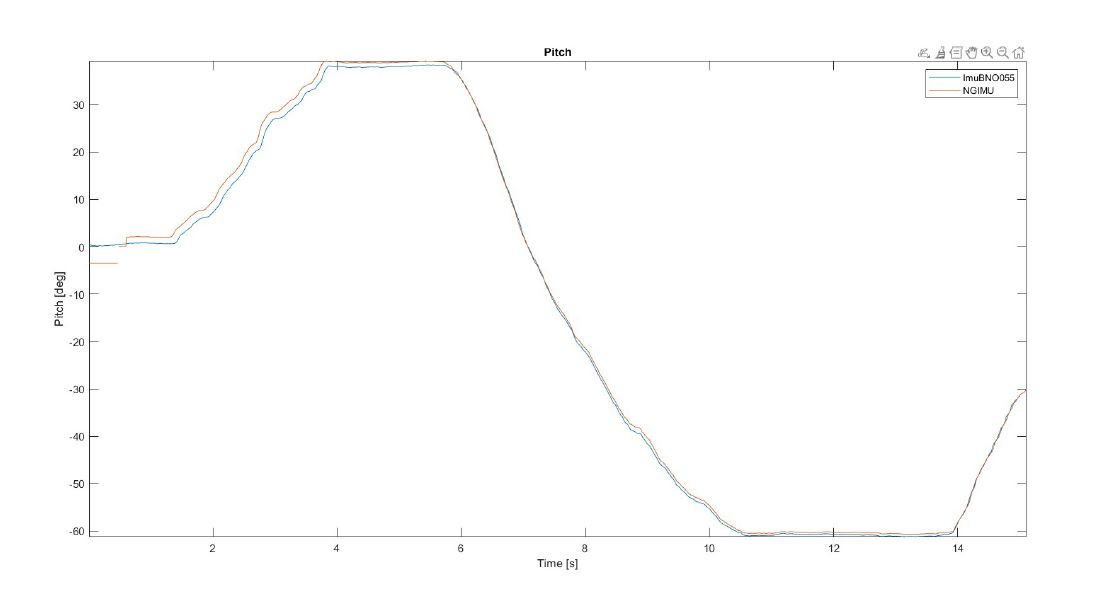
\includegraphics[width=0.8\textwidth,keepaspectratio]{figures/grafico.JPG}
\caption{Esempio di grafico}
\label{fig:grafico}
\end{figure}
\section{Test1}
Per ogni test riportate: cosa state testando, in che condizioni si è svolto il test, riferimenti a video/file di log che consegnate insieme a relazione e codice, grafici dei risultati, commento dei risultati.

\section{Test2}

\newpage
\addcontentsline{toc}{chapter}{Conclusioni e sviluppi futuri}
\section*{Conclusioni e sviluppi futuri}
Riassumere brevemente il lavoro svolto rispetto al task assegnato, evidenziando quali risultati sono stati raggiunti e quali no. Se ci sono aspetti del task non completati spiegare quali sono stati i problemi riscontrati in merito.\\
Inserire considerazioni personali su possibili sviluppi futuri dell'attività svolta (idee per migliorarla che non avete avuto modo di sperimentare, aspetti che suggerite di approfondire, problemi da risolvere..).

\addcontentsline{toc}{chapter}{Appendici}
\appendix
\chapter{Appendice1}
Se necessario ricorrete alle appendici per spiegare le parti "di contorno" dell'attività svolta e/o ciò che non riuscite ad inserire nello schema generale dei capitoli della relazione (es acquisizione dei dati con Matlab).


\bibliographystyle{ieeetr}
\bibliography{bibl} 
\end{document}
